% \usepackage{tikz}
% \usepackage{pgfplots}
% \pgfplotsset{compat=1.14}

\begin{figure}
    \centering
    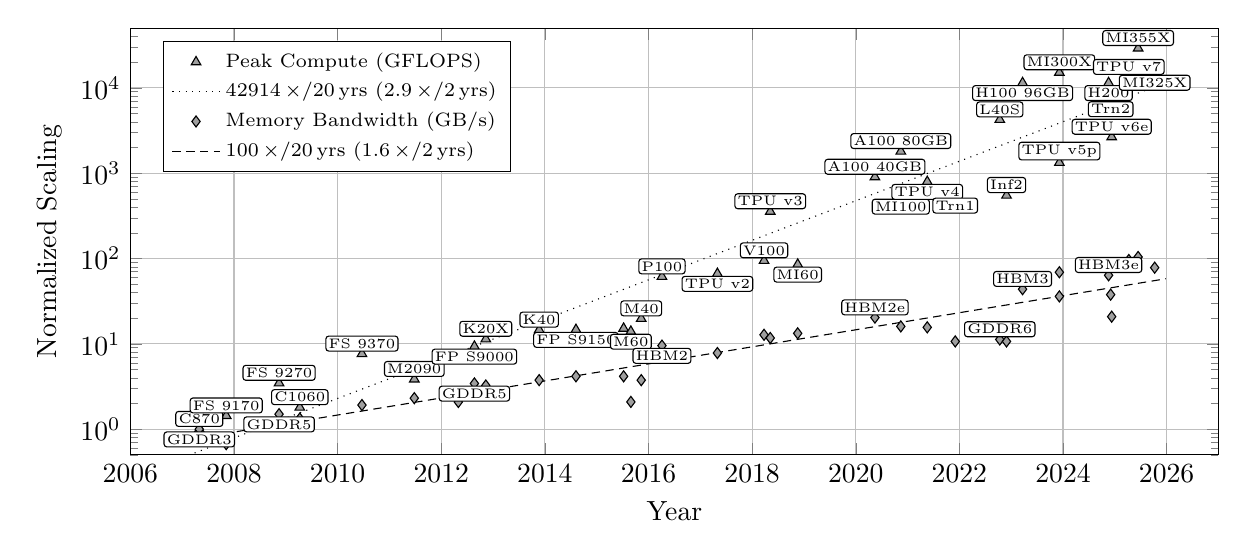
\begin{tikzpicture}
        \tikzstyle{lbl} = [font=\tiny, outer sep=1pt, fill=white, draw=black, inner sep=1pt, rounded corners=1pt]
        \begin{axis}[
            set layers,
            width=15.4cm,
            height=7cm,
            xlabel={Year},
            ylabel={Normalized Scaling},
            ymode=log,
            log basis y=10,
            ymin=0.5,
            ymax=50000.0,
            xmin=2006,
            xmax=2027,
            grid=major,
            minor grid style=dotted,
            scaled x ticks=false,
            xticklabel style={/pgf/number format/fixed, /pgf/number format/precision=0, /pgf/number format/1000 sep={}},
            legend pos=north west,
            legend cell align=left,
            legend style={font=\scriptsize},
        ]
            % ---------- Peak Compute (GFLOPS)
            \addplot [
                only marks,
                mark=triangle*,
                draw=none,
                fill=gray!75,
            ] coordinates {
                (2007.33, 1.0)
                (2007.85, 1.4389467592592593)
                (2008.87, 3.472222222222222)
                (2009.27, 1.8000578703703702)
                (2010.47, 7.638888888888888)
                (2011.48, 3.8547453703703702)
                (2012.33, 6.623263888888888)
                (2012.64, 9.33449074074074)
                (2012.86, 11.38599537037037)
                (2013.89, 14.600694444444443)
                (2014.6, 14.66724537037037)
                (2015.52, 15.156249999999998)
                (2015.66, 13.961226851851851)
                (2015.86, 19.768518518518515)
                (2016.26, 61.40046296296296)
                (2017.33, 66.55092592592592)
                (2018.23, 94.64699074074073)
                (2018.35, 355.90277777777777)
                (2018.88, 85.35879629629629)
                (2020.37, 902.3148148148148)
                (2020.87, 534.1435185185185)
                (2020.87, 1805.5555555555554)
                (2021.38, 795.7175925925925)
                (2021.92, 549.7685185185185)
                (2022.78, 4241.898148148148)
                (2022.91, 549.7685185185185)
                (2023.22, 11452.546296296296)
                (2023.93, 1328.125)
                (2023.93, 15132.523148148148)
                (2024.88, 11452.546296296296)
                (2024.92, 7416.087962962963)
                (2024.94, 2656.25)
                (2025.27, 13350.694444444443)
                (2025.45, 29127.02546296296)
                (2025.77, 15132.523148148148)
            };
            \addlegendentry{Peak Compute (GFLOPS)}

            % Regression line
            \addplot [
                dotted,
                domain=2007:2026,
                samples=200,
            ] { 0.01107113969714384 * 10^(0.23163004622153968 * (x - 2000))};
            \addlegendentry{42914\,$\times$/20\,yrs (2.9\,$\times$/2\,yrs)}

            % Data labels
            \begin{pgfonlayer}{axis descriptions}
                \node[lbl, anchor=south] at (axis cs:2007.33, 1.0) {C870};
                \node[lbl, anchor=south] at (axis cs:2007.85, 1.4389467592592593) {FS 9170};
                \node[lbl, anchor=south] at (axis cs:2008.87, 3.472222222222222) {FS 9270};
                \node[lbl, anchor=south] at (axis cs:2009.27, 1.8000578703703702) {C1060};
                \node[lbl, anchor=south] at (axis cs:2010.47, 7.638888888888888) {FS 9370};
                \node[lbl, anchor=south] at (axis cs:2011.48, 3.8547453703703702) {M2090};
                \node[lbl, anchor=north] at (axis cs:2012.64, 9.33449074074074) {FP S9000};
                \node[lbl, anchor=south] at (axis cs:2012.86, 11.38599537037037) {K20X};
                \node[lbl, anchor=south] at (axis cs:2013.89, 14.600694444444443) {K40};
                \node[lbl, anchor=north] at (axis cs:2014.6, 14.66724537037037) {FP S9150};
                \node[lbl, anchor=north] at (axis cs:2015.66, 13.961226851851851) {M60};
                \node[lbl, anchor=south] at (axis cs:2015.86, 19.768518518518515) {M40};
                \node[lbl, anchor=south] at (axis cs:2016.26, 61.40046296296296) {P100};
                \node[lbl, anchor=north] at (axis cs:2017.33, 66.55092592592592) {TPU v2};
                \node[lbl, anchor=south] at (axis cs:2018.23, 94.64699074074073) {V100};
                \node[lbl, anchor=south] at (axis cs:2018.35, 355.90277777777777) {TPU v3};
                \node[lbl, anchor=north] at (axis cs:2018.88, 85.35879629629629) {MI60};
                \node[lbl, anchor=south] at (axis cs:2020.37, 902.3148148148148) {A100 40GB};
                \node[lbl, anchor=north] at (axis cs:2020.87, 534.1435185185185) {MI100};
                \node[lbl, anchor=south] at (axis cs:2020.87, 1805.5555555555554) {A100 80GB};
                \node[lbl, anchor=north] at (axis cs:2021.38, 795.7175925925925) {TPU v4};
                \node[lbl, anchor=north] at (axis cs:2021.92, 549.7685185185185) {Trn1};
                \node[lbl, anchor=south] at (axis cs:2022.78, 4241.898148148148) {L40S};
                \node[lbl, anchor=south] at (axis cs:2022.91, 549.7685185185185) {Inf2};
                \node[lbl, anchor=north] at (axis cs:2023.22, 11452.546296296296) {H100 96GB};
                \node[lbl, anchor=south] at (axis cs:2023.93, 1328.125) {TPU v5p};
                \node[lbl, anchor=south] at (axis cs:2023.93, 15132.523148148148) {MI300X};
                \node[lbl, anchor=north] at (axis cs:2024.88, 11452.546296296296) {H200};
                \node[lbl, anchor=north] at (axis cs:2024.92, 7416.087962962963) {Trn2};
                \node[lbl, anchor=south] at (axis cs:2024.94, 2656.25) {TPU v6e};
                \node[lbl, anchor=south] at (axis cs:2025.27, 13350.694444444443) {TPU v7};
                \node[lbl, anchor=south] at (axis cs:2025.45, 29127.02546296296) {MI355X};
                \node[lbl, anchor=north] at (axis cs:2025.77, 15132.523148148148) {MI325X};
            \end{pgfonlayer}

            % ---------- Memory Bandwidth (GB/s)
            \addplot [
                only marks,
                mark=diamond*,
                draw=none,
                fill=gray!75,
            ] coordinates {
                (2007.33, 1.0)
                (2007.85, 0.668359375)
                (2008.87, 1.5)
                (2009.27, 1.3333333333333335)
                (2010.47, 1.9166666666666665)
                (2011.48, 2.3098958333333335)
                (2012.33, 2.0833333333333335)
                (2012.64, 3.4375)
                (2012.86, 3.25)
                (2013.89, 3.755208333333333)
                (2014.6, 4.166666666666667)
                (2015.52, 4.166666666666667)
                (2015.66, 2.088541666666667)
                (2015.86, 3.755208333333333)
                (2016.26, 9.533854166666668)
                (2017.33, 7.8125)
                (2018.23, 12.7734375)
                (2018.35, 11.71875)
                (2018.88, 13.28125)
                (2020.37, 20.3125)
                (2020.87, 16.015625)
                (2020.87, 26.549479166666668)
                (2021.38, 15.625)
                (2021.92, 10.677083333333334)
                (2022.78, 11.25)
                (2022.91, 10.677083333333334)
                (2023.22, 43.75)
                (2023.93, 36.00260416666667)
                (2023.93, 69.01041666666667)
                (2024.88, 63.671875)
                (2024.92, 37.76041666666667)
                (2024.94, 20.833333333333336)
                (2025.27, 96.09375)
                (2025.45, 104.16666666666667)
                (2025.77, 78.125)
            };
            \addlegendentry{Memory Bandwidth (GB/s)}

            % Regression line
            \addplot [
                densely dashed,
                domain=2007:2026,
                samples=200,
            ] { 0.14676174382859433 * 10^(0.0999131879159643 * (x - 2000))};
            \addlegendentry{100\,$\times$/20\,yrs (1.6\,$\times$/2\,yrs)}

            % Data labels
            \begin{pgfonlayer}{axis descriptions}
                \node[lbl, anchor=north] at (axis cs:2007.33, 1.0) {GDDR3};
                \node[lbl, anchor=north] at (axis cs:2008.87, 1.5) {GDDR5};
                \node[lbl, anchor=north] at (axis cs:2012.64, 3.4375) {GDDR5};
                \node[lbl, anchor=north] at (axis cs:2016.26, 9.533854166666668) {HBM2};
                \node[lbl, anchor=south] at (axis cs:2020.37, 20.3125) {HBM2e};
                \node[lbl, anchor=south] at (axis cs:2022.78, 11.25) {GDDR6};
                \node[lbl, anchor=south] at (axis cs:2023.22, 43.75) {HBM3};
                \node[lbl, anchor=south] at (axis cs:2024.88, 63.671875) {HBM3e};
            \end{pgfonlayer}

        \end{axis}
    \end{tikzpicture}

    \caption{Development of Peak Compute vs. Memory Bandwidth}
    \label{fig:memory_wall_problem}
\end{figure}
